%%\chapter{\textit{Python}}%%

pada bab in yang akan di bahas yaitu mengenai sejarah singkat dari \textit{Framework CodeIgniter}, kemudian keunggulan dari \textit{Framework CodeIgniter},
kemudian sarana untuk memperajari \textit{Framework CodeIgniter}, kemudian alat pendukung untuk menggunakan \textit{Framework CodeIgniter} lalu dilanjutkan dengan penjelasan singkat tentang MVC 
pada \textit{Framework CodeIgniter} setelah itu penjelasan tentang direktori pada paket yang telah di sediakan oleh \textit{Framework CodeIgniter}, terakhir merupakan editor teks yang dianjurkan
 untuk \textit{Framework CodeIgniter} serta contoh implementasi MVC sederhana.\pagebreak

\section{Sejarah \textit{CodeIgniter}}
Codeigniter merupakan \textit{faramework} web yang digunakan untuk bahasa pemerograman PHP yang dibuat oleh Rick Ellis pada tahun 2006 tepatnya pada tanggal 28 Febuari 2006,  penemu dan pendiri Ellis Lab (www.ellislab.com). Ellislab merupakan suatu tim kerja yang berdiri pada tahun 2002 dan bergerak di bidang pembuatan software dan tool untuk para pengembang web. Kemudian pada bulan Juli 2013 Ellis Lab mereka mengumumkan mencari pemilik baru untuk \textit{CodeIgniter} yang dikarenakan pada lingkup internal tidak memiliki fokus untuk mengembangkan \textit{CodeIgniter}, kemudian pada tahun 2014 tepatnya pada bulan oktober 2014 sampai sekarang, EllisLab telah menyerahkan hak kepemilikan \textit{CodeIgniter} ke \textit{British Columbia Institute of Technology} (BCIT) yang merupakan sekolah tinggi teknologi di kanada, untuk proses pengembangan lebih lanjut. Saat ini situs resmi \textit{CodeIgniter} telah berubah dari \textit{www.ellislab.com} ke \textit{www.codeigniter.com.} \cite{raharjo2015belajar}. \par

Setelah kurang lebih lima bulan setelah berpindah kepemilikan, BCIT akhirnya merilis \textit{CodeIgniter} versi 3.0, yang jika dibandingkan dengan versi sebelumnya tentunya \textit{CodeIgniter} 3 memiliki fitur yang lebih kaya seperti pengembangan \textit{database driver}, terdapat pustaka-pustaka baru dan juga PDO \textit{CodeIgniter} yang telah berfungsi secara penuh dengan subdriver \cite{subagia2018kolaborasi}.\par

Dibandingkan web \textit{faramework} yang lain \textit{CodeIgniter} memiliki desain yang lebih sederhana dan bersifat tidak kaku (fleksibel). \textit{CodeIgniter} masih mengizinkan atau memberikan kebebasan kepada para pengembang untuk menulis code-code tertentu di dalam aplikasi menggunakan cara konvesional atau tanpa menggunakan \textit{faramework} \cite{david2017codeigniter}.\par

Ditulis padadokumentasi \textit{CodeIgniter}, \textit{CodeIgniter} juga merupakan tollkit bagi orang atau perogramer yang ingin membangun aplikasi web menggunakan PHP. Tujuannya adalah membuat pengembangan proyek menjadi lebih cepat daripada membuat code dari awal. Pada \textit{CodeIgniter} juga memberikan kumpulan library untuk program yang sering di gunakan dan untuk mengakses library tersebut terbilang cukup mudah, dengan menggunakan framework codeigniter kita tinggal fokus pada pengembangan sistem atau projek serta meminimalisir jumlah kode yang akan dibuat.\pagebreak

\section{Beberapa Keuntungan \textit{CodeIgniter}}
CodeIgniter merupakan toolkit untuk orang-orang yang ingin membuat atau membangun aplikasi web menggunakan bahasa pemerograman PHP. Adapun beberapa keunggulan yang di tawarkan oleh CodeIgniter adalah sebagai \cite{raharjo2015belajar} , \cite{subagia2018kolaborasi} berikut:\par

\begin{enumerate}
\item \textit{CodeIgniter} merupakn framework yang bersipat gratis atau open-source
\item \textit{CodeIgniter} memiliki ukuran file yang relatif kecil dibandingkan Framework php lain. Setelah di download dan di ekstrak file codeigniter memiliki total ukuran kurang lebih 11 MB dengan ketentuan folder user guide (dokumentasi \textit{CodeIgniter}) kurang lebih sebesar 9 MB dan folder aplikasi dan sistem dengan ukurang kurang lebih 2 MB 
\item Aplikasi yang dibuat menggunakan codeigniter dapat berjalan dengan cepat
\item \textit{CodeIgniter} Menggunakan pola desain Model-View-Controller (MVC) yang memungkinkan pada satu file tidak akan berisi banyak code. Halini mengakibatkan kode menjadi mudah untuk di baca, dipahami dan dikembangkan atau dilakukan maintaining (pemeriharaan) di kemudian hari.
\item \textit{CodeIgniter} dapat diperluas sesuai dengan kebutuhan.
\item \textit{CodeIgniter} juga terdokuntasi dengan baik atau memiliki dokumentasi yang sangat baik. Informasi tentang class dan function yang terdapat pada codeigniter dapat diperoleh melalui dokumentasi yang disediakan pada paket distribusinya.
\item \textit{Pack a Punch}, \textit{CodeIgniter} hadir dengan \textit{library} yang akan membantu tugas-tugas di pengembangan web yang sudah umum dan sering di lakukan seperti mengakses basis data, mengirim email, validasi data dari form, mengelola session, memanipulasi gambar,  dan masih banyak lagi yang lainnya.
\item \textit{Extensible}kita dapat menambahkan \textit{library} atau \textit{helper} yang di ciptakan sendiri kemudian di terapkan pada \textit{CodeIgniter}. selain itu bisa juga ditambahkan melalui \textit{class ekstension} atau sistem \textit{sistem hooks} 
\end{enumerate}

\section{Persiapan Untuk Menggunakan \textit{CodeIgniter}}

CodeIgniter merupakan framework PHP. Untuk dapat menggunakan terlebih dahulu programmer harus sudah familiar dengan penggunaan bahasa pemerograman PHP atau sudah mahir menggunakan bahasa pemerograman PHP. Selain itu, CodeIgniter merupakan framework yang memiliki konsep MVC maka pada saat melakukan pemerograman menggunakan framework CodeIgniter pasti bersinggungan dengan model, view dan controller dimana isi dari model dan controller merupakan class yang merupakan inti dari pemerograman yang berorientasi objek. Maka dari itu untuk menggunakan codeigniter harus mengetahui konsep pemerograman berorientasi objek menggunakan PHP.\par

\section{ Tools yang Dugunakan}
Untuk dapat menggunkan \textit{CodeIgniter} setidaknya harus terlebih dahulu memiliki beberapa tolls berupa aplikasi yang teristall pada komputer yang akan digunakan untuk pemerograman adapun tolls yang digunakan agar bisa menggunakan \textit{Framework CodeIgniter} diantaranya\par

\subsection{PHP}
	php merupakan bahasa pemerograman yang digunakan yang di gunakan sebagai base pada \textit{CodeIgniter} oleh karena itu bahasa pemerograman PHP harus terinstall terlebih dahulu pada komputer yang akan dilakukan pemerograman sehingga \textit{Framework CodeIgniter} dapat digunakan, pada buku ini PHP yang digunakan merupakan PHP 5 dikarenakan pada buku ini masih menggunakan library yang berkaitan dengan PHP 5.\par

\subsection{Web Server}
Web server atau server web merupakan tool yang digunakan untuk mengeksekusi code PHP sehingga hasil dari code PHP tersebut dapat terlihat, sedangkan web server yang di gunakan merupakan apache. Merupakan web server lokal yang harus di istall pada komputer yang akan digunakan untuk pemerograman, jika apache telah terinstall jalankan terlebih dahulu apache tersebut kemudian pada web browser isikan alamat localhost atau bisa dengan mengisikan alamat IP 127.0.0.1\par

\subsection{Server Database }
Setelah web server swlanjutnya yaitu Server database yang merupakan database atau pusat penyimpanan data dari web yang di buat, biasanya server database yang sering di gunakan merupakan database MySql, selain dari database MySql juga dapat di gunakan yang penting database tersebut termasuk pada jenis database yang dapat di hubungkan melalui Open Database Connectivity (ODBC).\par

selain dari ketiga opsi tersebut ada pilihan lain dalam menginstall ke tiga tools tersebut dapat menggunakan XAMPP, XAMPP merupakan aplikasi yang di dalammya terdapat dari kumpulan aplikasi yang digunakan untuk pengembangan dan pembuatan website berupa Apache, MySQL, PHP, dan Perl, dengan menggunakan XAMPP dapat mempersingkat pekerjaan yang tadinya harus menginstall PHP, Apache, dan MySQL secara terpisah menjadi satu, hanya dengan menggunakan satu aplikasi XAMPP semua aplikasi tersebut telah teristall. 

\textbf{Catatan :}\par
\textit{Untuk xampp dari versi 5 sampai 7 sekarang sudah tidak menggunakan database MySQL melainkan menggunakan database MariaDB, namun tidak perlu kawathir dikarenakan MariaDB basenya masih Menggunakan MySQL.}\pagebreak

\subsection{Instalasi XAMPP}
Dikarenakan ketiga tolls pendukung Untuk \textit{CodeIgniter} dapat di satukan dalam paket yang telah di sediakan XAMPP maka agar lebih mudah, maka pada penjelasan di buku ini untuk instalasi Toll pendukung menggunakan XAMPP, maka dari itu pada sub bab ini dijelaskan cara installasi XAMPP. adapun untuk langkah-langkah istalasi beserta screenshot sebagai berikut:

\begin{enumerate}


\item Langkah pertama untuk instalasi xampp yaitu Unduh terlebih dahulu File XAMPP pada laman website resmi dari xampp pada alamat berikut\par
https://www.apachefriends.org/download.html.

\item pilih xampp versi 5 agar PHP yang di gunakan merupakan PHP 5, kemudian jika file tersebut telah di unduh maka hasil filenya seperti pada gambar \ref{x1}

\begin{figure}[htbp]
	\centerline{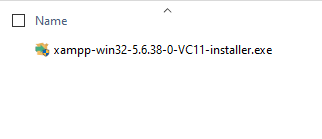
\includegraphics[width=0.50\textwidth]{figures/xampp/hasil.png}}
	\caption{Xampp exe}
	\label{x1}
\end{figure}

\item Kemudian setelah itu jalankan file tersebut dengan cara klik kanan pilih run administrator seperti pada gambar \ref{x2} berikut 

\begin{figure}[!htbp]
	\centerline{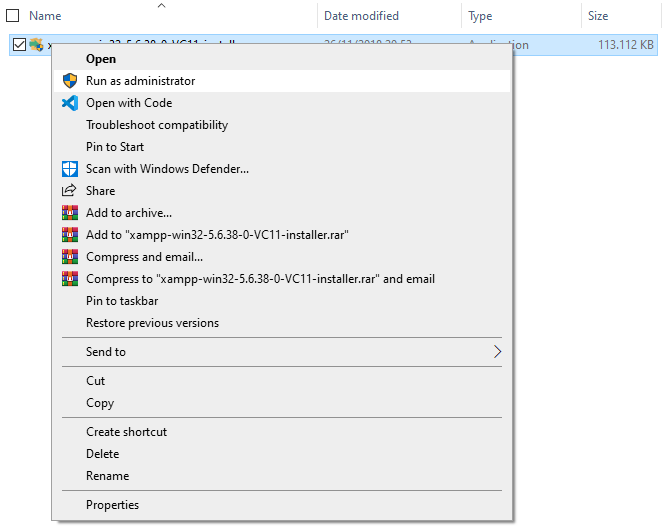
\includegraphics[width=0.60\textwidth]{figures/xampp/1.png}}
	\caption{Run Administrator Xampp}
	\label{x2}
\end{figure}
\pagebreak

\item Kemudan jika muncul popup pilihan untuk memasang aplikasi pada komputer pilih yes, lalu tunggu beberapa saat maka akan muncul setup XAMPP separti pada gambar \ref{x3}.

\begin{figure}[!htbp]
	\centerline{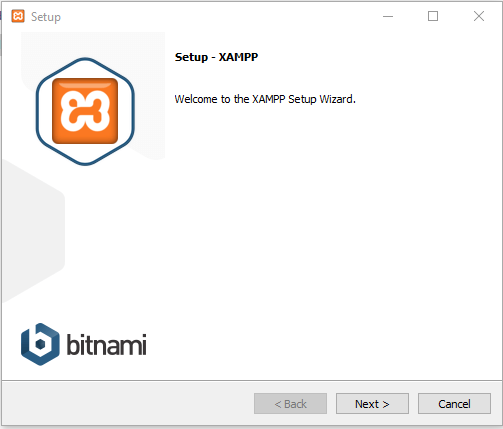
\includegraphics[width=0.70\textwidth]{figures/xampp/2.png}}
	\caption{Setup Xampp}
	\label{x3}
\end{figure}

\item Kemudian klik Next untuk melanjutkan peroses Instalasi \ref{x3}


\begin{figure}[!htbp]
	\centerline{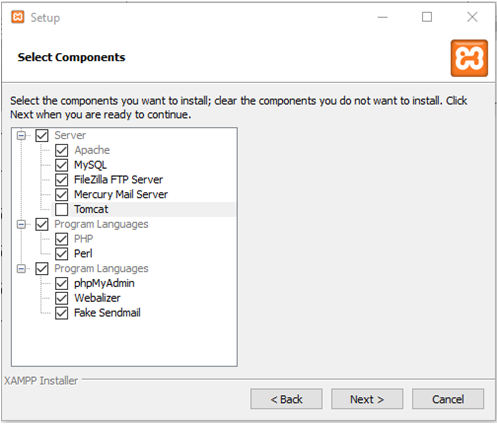
\includegraphics[width=0.70\textwidth]{figures/xampp/3.png}}
	\caption{Memilih Komponen Xampp}
	\label{x4}
\end{figure}

\item Pada gambar \ref{x4} merupakan peroses memilih software yang akan di pasang pada komputer sebagai contoh hilangkan tanda checklist pada check box Tomcat, kemudian kelik tombol Next.

\begin{figure}[!htbp]
	\centerline{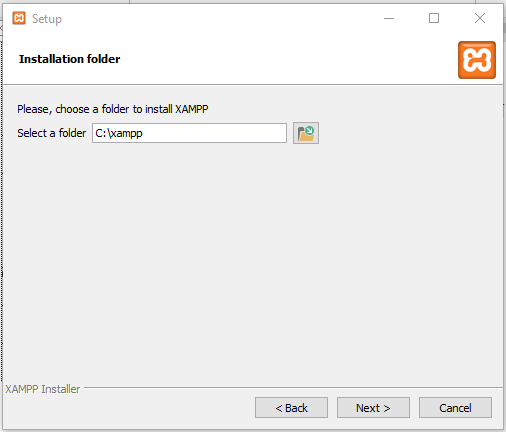
\includegraphics[width=0.70\textwidth]{figures/xampp/4.png}}
	\caption{Tempat Istall Xampp}
	\label{x5}
\end{figure}


\item Pada gambar \ref{x5} merupakan menentukan tujuan instalasi XAMPP, secara default xampp akan teristal pada direktori C:xampp, jika tidak akan menginstall di direktori C maka datapat memilih direktori lain dengan cara klik tmbol browser yang bergambar folder dengan anak panah. Kemudian klik tombol Next untuk melanjutkan peroses.
\pagebreak
\begin{figure}[!htbp]
	\centerline{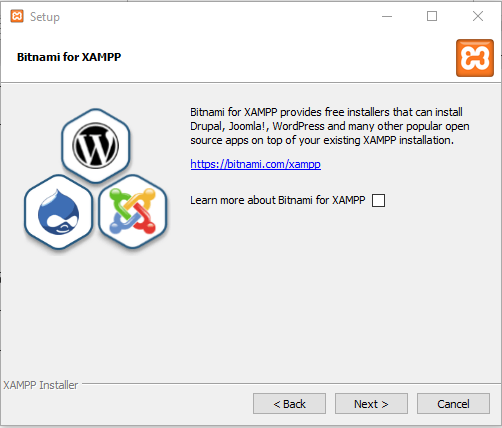
\includegraphics[width=0.70\textwidth]{figures/xampp/5.png}}
	\caption{Bitami Untuk Xampp}
	\label{x6}
\end{figure}


\item Pada gambar \ref{x6} uncheck checklist yang terdapat pada halaman tersebut, kemudian klik tombo Next untuk melanjutkan peroses installasi.
 
\begin{figure}[!htbp]
	\centerline{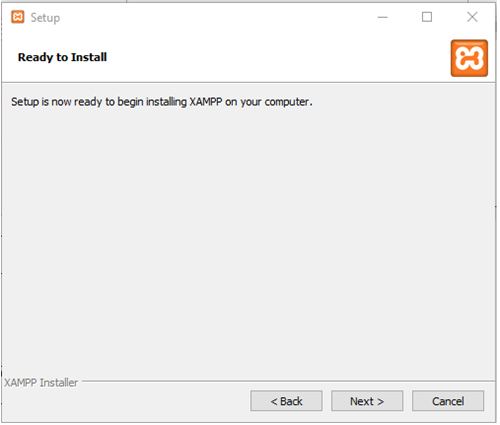
\includegraphics[width=0.70\textwidth]{figures/xampp/6.png}}
	\caption{Xampp Siap diinstal}
	\label{x7}
\end{figure}
 
\item Pada gambar \ref{x7} menunjukan bahwa semua aplikasi yang telah di cheklis tadi dan telah di tentukan tempat installnya, telah siap untuk diinstal, kemudian klik tombol Next untuk melanjutkan proses instal
 


\item Pada gambar \ref{x8} menunjukan peroses install aplikasi pada peroses ini tunggu instal aplikasinya beres jika muncul popup klik finish untuk mengakhiri proses istalasi
\begin{figure}[!htbp]
	\centerline{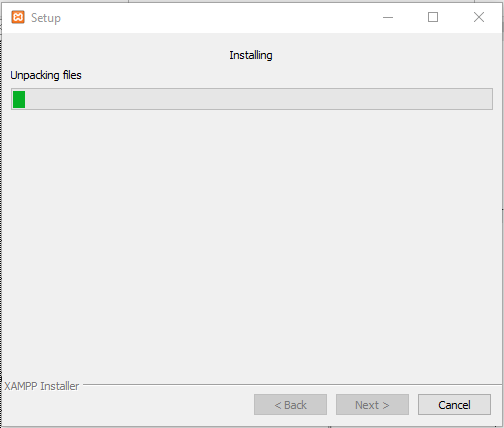
\includegraphics[width=0.70\textwidth]{figures/xampp/7.png}}
	\caption{Proses Install Xampp}
	\label{x8}
\end{figure}

\item pada gambar \ref{x9} tersebut kemudian klik tombol open untuk memunculkan XAMPP control panel
\begin{figure}[!htbp]
	\centerline{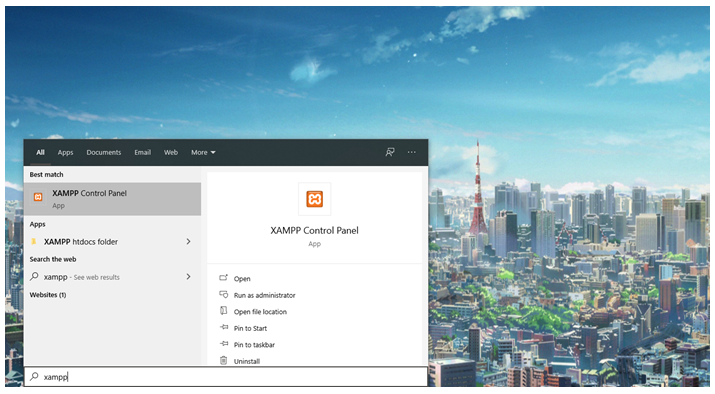
\includegraphics[width=1\textwidth]{figures/xampp/8.png}}
	\caption{Membuaka Xampp}
	\label{x9}
\end{figure}

\item pada gambar \ref{x10} tersebut jalankan service apache dan MySQL dengan cara klik tombol start yang terdapat di sebelah tulisan apache dan MySQL.
\begin{figure}[!htbp]
	\centerline{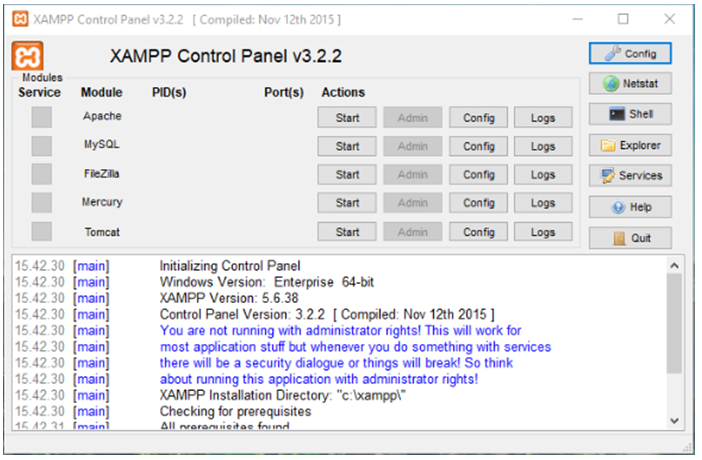
\includegraphics[width=1\textwidth]{figures/xampp/9.png}}
	\caption{Control Panel Xampp}
	\label{x10}
\end{figure}
\end{enumerate}
\textbf{Catatan :}\par
\textit{Untuk melatekan dokumen codeigniter pada xampp dapat di simpan pada dokumen root apache yang terletak pada Direktori C pada folder xampp di subfolder htdocs }\pagebreak


%% editor teks 
\section{ Editor Text yang Digunakan}
	Setelah xampp terinstall, maka selanjutnya di butuhkan editor text yang digunakan untuk membuat souce code atau kode baik itu php, html, java script dan lainnya, untuk editor text itu sendiri banyak ragamnya seperti notepad++, SublimeText 3, atom dan lain-lain, terkhusus pada buku ini untuk tolls editor teksnya menggunakan visual studio code yang merupakan editorteks yang di liris oleh  microsoft dan editor teks ini gratis.

\subsection{Kelebihan dari Visual Studio Code}
Adapun kelebihan dari editor teks visual studio code yaitu:
\begin{enumerate}
\item dapat di gunakan pada semua sistem operasi yaitu windows, linux, dan macos
\item banyak menyediakan ekstensi sehingga mempermudah dalam melakukan pembuatan kode
\item dapat terintegrasi dengan git 
\item dapat membuka terminal atau comand from pada aplikasi visual studio code
\end{enumerate}

\subsection{Instalasi Visual Studio Code}
	pada peroses instalasi visual studio code dilakukan untuk sistem operasi windows, kemudian untuk menerapkan visual studio code pada sistem operasi windows dapat mengikuti tahapan-tahapan seperti berikut:
\begin{enumerate}
\item Unduh terlebih dahulu visual studio code pada website resminya pada alamat berikut https://code.visualstudio.com/ untuk halaman utama website tersebut seperti pada gambar \ref{V1} berikut:\par
 \begin{figure}[!htbp]
	\centerline{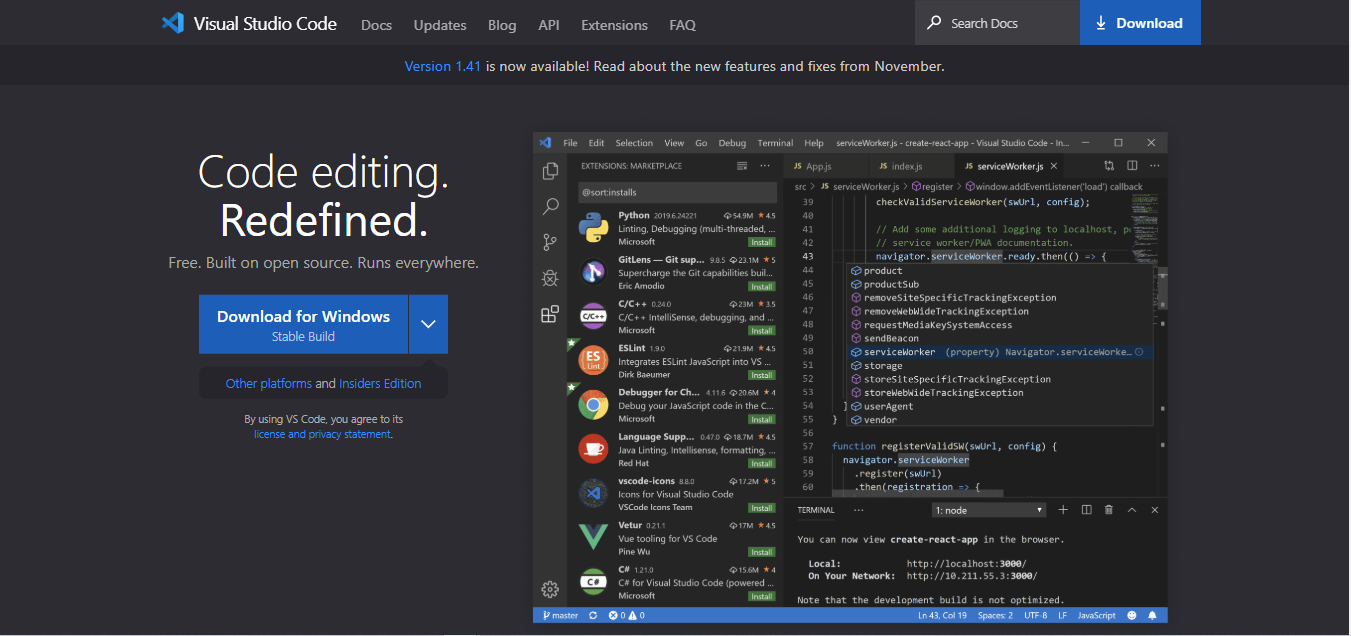
\includegraphics[width=0.90\textwidth]{figures/vs/1.png}}
	\caption{Halaman Utama Website Visual Studio Code}
	\label{V1}
\end{figure}
\item jika telah muncul tampilan seperti gambar \ref{V1} pilih tombol download for windows yang terdapat pada sebelah kiri halaman tersebut, jika yang munculnya bukan pilihan download for windows bisa dicari dengancara menekan tombol panah yang terdapat disebelah tombol download forwindows, hal ini juga bisa dilakukan jika ingin mengunduh visual studio code untuk sistem oprasi linux atau mac, untuk detail pilihan untuk opsi download seperti pada gambar \ref{V2}.\par

\begin{figure}[!htbp]
	\centerline{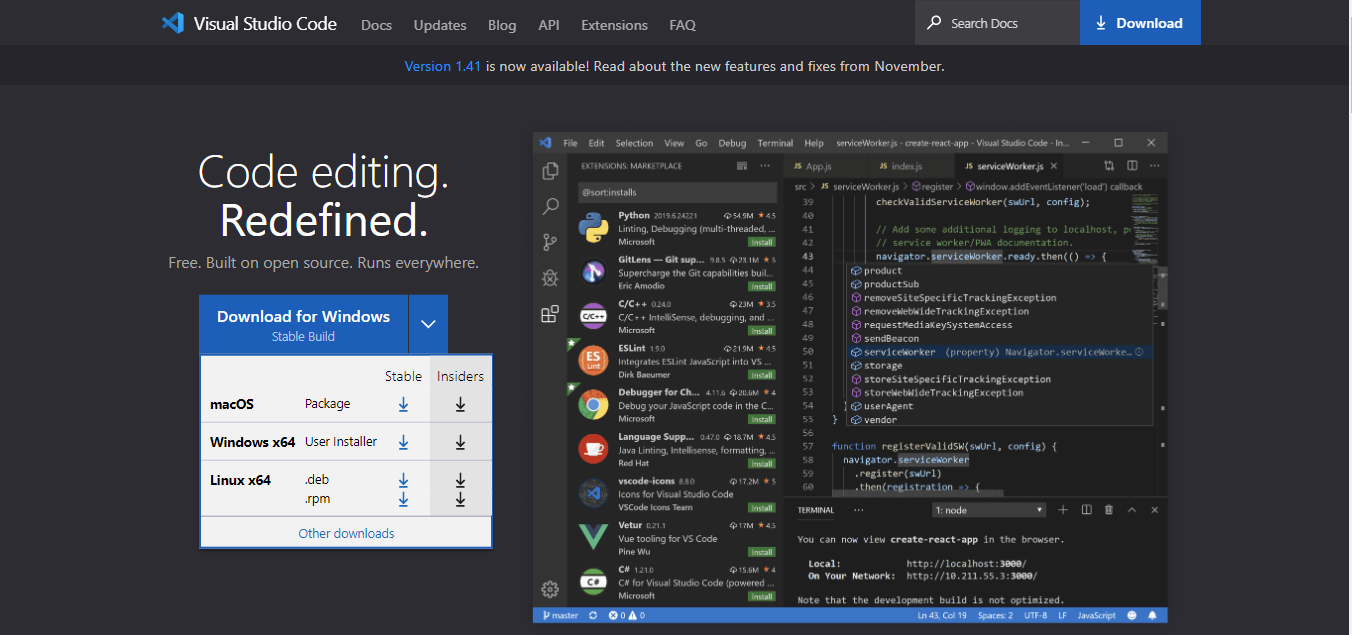
\includegraphics[width=0.9\textwidth]{figures/vs/2.png}}
	\caption{Memilih Visial Studio Berdasarkan OS}
	\label{V2}
\end{figure}
 
\item dikarenakan pada projek yang akan di bahas pada buku ini menggunakan sistem operasi windows sehingga pada tampilan di gambar \ref{V2} pilih visual studio for windows kemudian unduh file tersebut\par 

\begin{figure}[!htbp]
	\centerline{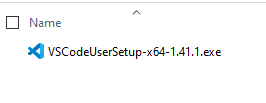
\includegraphics[width=0.6\textwidth]{figures/vs/3.png}}
	\caption{File exe visual studio code}
	\label{V3}
\end{figure}

\item Jika sudah di unduh maka hasil unduhnya berupa file exe seperti pada gambar \ref{V3} dimana file tersebut akan di jalankan agar visual studio dapat di terapkan pada komputer atau laptop yang akan di gunakan untuk pemerograman.\par

\item Pada Gambar \ref{V4} merupakan peroses awal untuk instalasi visual code dengan cara klik kanan pilih Run as administrator atau degan cara klik duakali pada file visual studio code lalu tngggu beberapa saat, jika munul notifikasi berupa pop up klarifikasi untuk install aplikasi, pilih yes untuk melanjutkan proses.\par \pagebreak
\begin{figure}[!htbp]
	\centerline{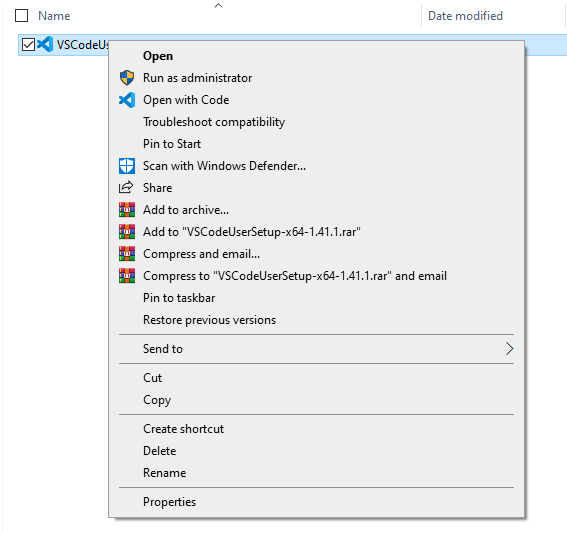
\includegraphics[width=0.6\textwidth]{figures/vs/4.png}}
	\caption{Run Administrator}
	\label{V4}
\end{figure}

\item Pada gambar \ref{V5} merupakan pilihan lisensi atau ketentuandari visual studio code, pada tampilan ini pilih I accept the agreement yang merupakan perintah bahwa menyetujui ketentuan yang di berikan untuk pemasangan aplikasi visual studio code setelah itu klik tombol Next, untuk melanjutkan peroses instalasi.
 \begin{figure}[!htbp]
	\centerline{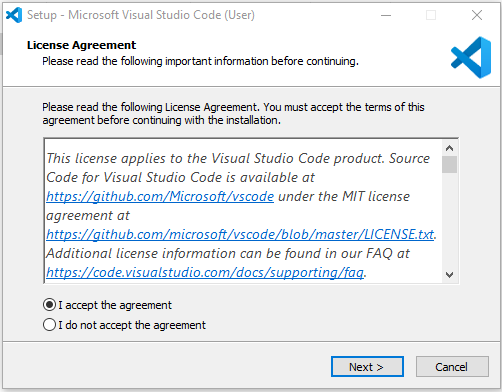
\includegraphics[width=0.80\textwidth]{figures/vs/5.png}}
	\caption{Persetujuan Lisensi}
	\label{V5}
\end{figure}

\item Pada gambar \ref{V6}  merupakan opsi untuk tempat di installnya aplikasi visual studio code secara default visual studio code akan terinstal di direktori 
\begin{verbatim} C:\User\nama_user\AppData\Local\Programs
\Microsoft VS Code 
\end{verbatim}
 jika ingin memilih opsi lain dapat memilih tombol Browse… kemudian memilih folder tempat di installnya visual studio code, jika telah selesai klik tombol Next untuk melanjutkan proses install
\begin{figure}[!htbp]
	\centerline{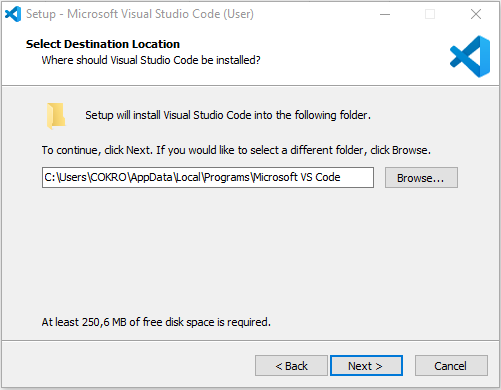
\includegraphics[width=0.90\textwidth]{figures/vs/6.png}}
	\caption{Direktori Visual Code Di install}
	\label{V6}
\end{figure}
 \pagebreak
\item Pada gambar \ref{V7} merupakan opsi untuk memilih start menu, jika telah memilih start menu maka klik Next untuk melanjutkan proses install

\begin{figure}[!htbp]
	\centerline{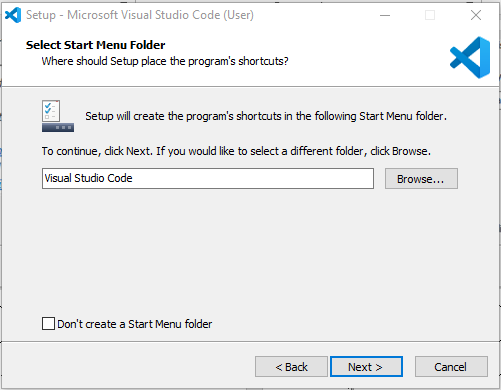
\includegraphics[width=0.90\textwidth]{figures/vs/7.png}}
	\caption{Memilih Start Menu}
	\label{V7}
\end{figure}
\item Pada gambar \ref{V8}  merupakan opsi untuk menembahkan taks, dengan di tambahkannya taks maka untuk membuka file pemerograman bisa dengan klik kanan pada file pemerograman kemudian open with visual code, tidak hanaya itu dengan di ceklisnya taks pada pilihan tersebut file yang berekstensi php,html, dan lainnya yang berekstensi kode pemerograman akan memiliki icon sesuai dengan ekstensi dari file tersebut, kemudian pada taks PATH agar visual code bisa mengakses comand from atau terminal, untuk rekomendasi taks yang harus di pilih dapat dilihat pada gambar \ref{V8}. jika suadah dipilih sesuai dengan gambar maka bisa dilanjutkan dengan menekan atau klik tombol Next, untuk melanjutkan proses istall visual code.
 \pagebreak
\begin{figure}[!htbp]
	\centerline{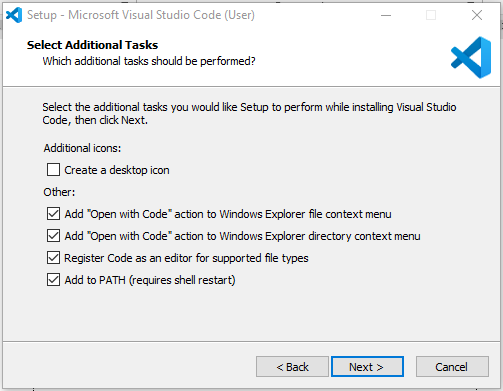
\includegraphics[width=0.80\textwidth]{figures/vs/8.png}}
	\caption{Menambahkan Taks}
	\label{V8}
\end{figure}

\begin{figure}[!htbp]
	\centerline{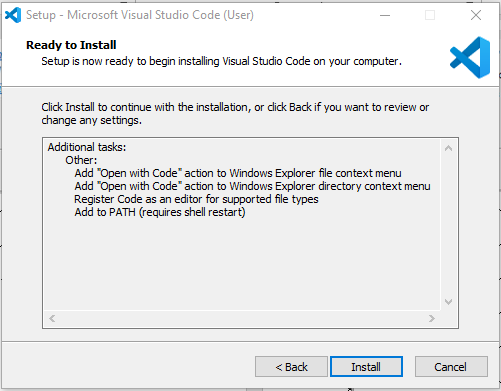
\includegraphics[width=0.80\textwidth]{figures/vs/9.png}}
	\caption{Visual Studio Siap Di Install}
	\label{V9}
\end{figure}

\item Kemudian Pada gambar \ref{V9} menunjukan bahwa visual studio code telah siap untuk di install, klik Install untuk melanjutkan proses install visual studio code. 



\item Pada gambar \ref{V10} merupakan peroses install aplikasi, pada proses ini tunggu sekitar 5 menit jika telah selesai maka akan muncul gambar seperti pada gambar \ref{V10} berikut.

\begin{figure}[!htbp]
	\centerline{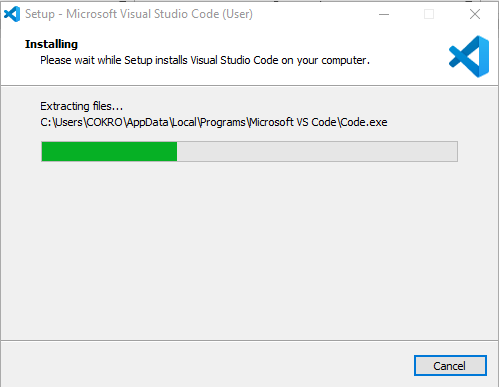
\includegraphics[width=0.70\textwidth]{figures/vs/10.png}}
	\caption{Proses Install Visual Code}
	\label{V10}
\end{figure}

\item Setelah muncul seperti gambar \ref{V11} kemudian klik finish untuk mengakhiri proses instalasi visual studio code. 
\begin{figure}[!htbp]
	\centerline{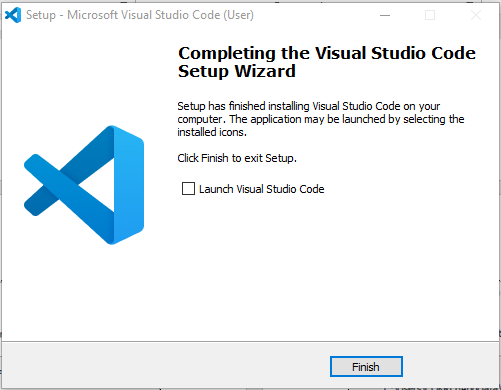
\includegraphics[width=0.70\textwidth]{figures/vs/11.png}}
	\caption{Visual Studio Selesai Di Install}
	\label{V11}
\end{figure}
 
\item Untuk dapat menjalankan visual studio code dapat dengan cara klik icon search yang berada di dekat icon vindows yang berada pada task bar kemudian tekan dan ketik visual maka muncul visual tudio code dan klik open untuk menjalankan visual studio code untuk jelasnya seperti pada gambar \ref{V12}. 

\begin{figure}[!htbp]
	\centerline{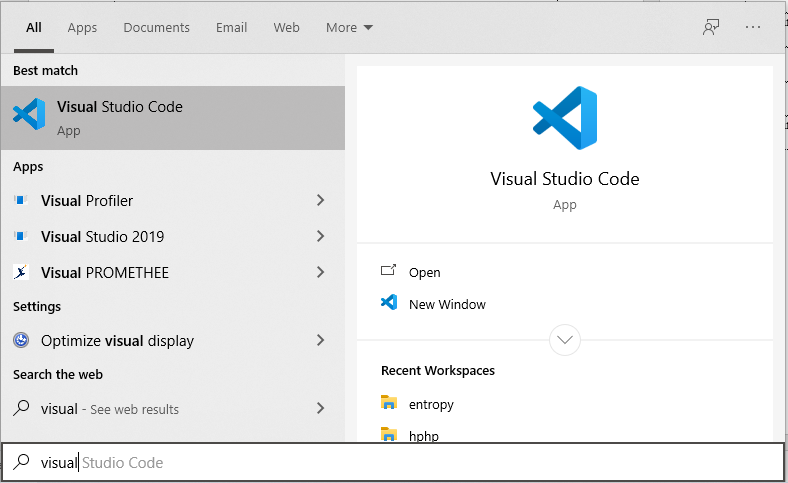
\includegraphics[width=0.90\textwidth]{figures/vs/12.png}}
	\caption{Mencari Visual Studio}
	\label{V12}
\end{figure}


\item Pada gambar \ref{V13} merupakan tampilan awal visual studio code jika telah selesai di install.
\begin{figure}[!htbp]
	\centerline{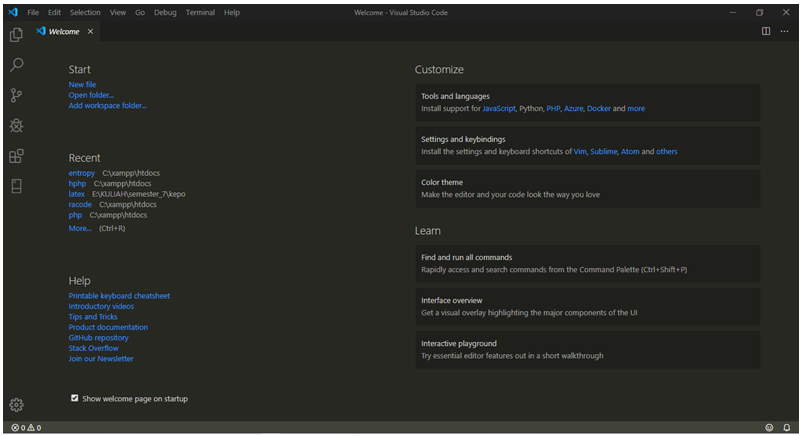
\includegraphics[width=0.90\textwidth]{figures/vs/13.png}}
	\caption{Tampilan Awal Visual Studio}
	\label{V13}
\end{figure}

\item Pada gambar \ref{V14}  merupakan menu untuk memilih ekstensi yang dapat di terapkan pada visual studio code.\par
\begin{figure}[!htbp]
	\centerline{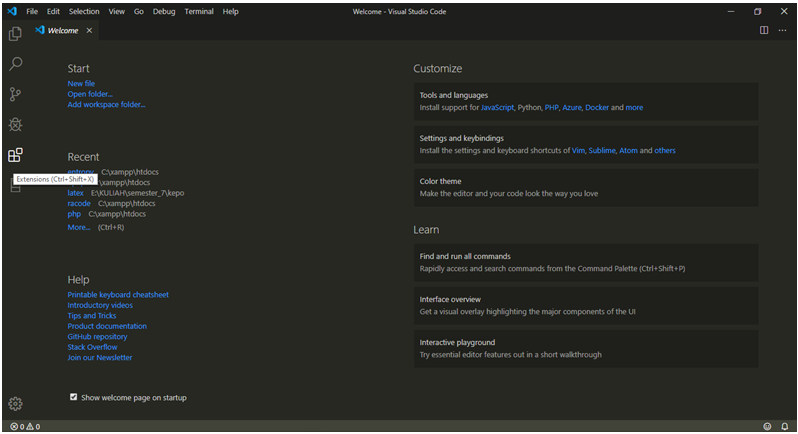
\includegraphics[width=0.90\textwidth]{figures/vs/14.png}}
	\caption{Menu Ekstensi Visual Studio}
	\label{V14}
\end{figure}
\pagebreak

\end{enumerate}


\subsection{Ekstensi Visual Studio Code}

Ekstensi merupakan tolls tambahan yang di gunakan pada aplikasi, adapun pada visual studio code ekstensi yang di gunakan merupakan tambahan tolls untuk membantu dalam pembuatan souce code, dengan di tambahkannya ekstensi pada visual studio code maka dalam pembuatan source code menjadi lebih cepat dan mudah, dikarenakan dengan di tambahkannya ekstensi source code yang error dapat terdeteksi kemudian jika kita akan menulis suatu code hanya perlu menuliskan dua atau tiga huruf pertama kemudian dengan ekstensi tersebut akan di rekomendasikan code yang akan di gunakan. maka dari itu pada buku ini projek yang di buat menggunakan teks editor visual studio code, adapun tambahan ekstensi yang di gunakan agar menunjang projek yang dilakukan pada buku ini adalah sebagai berikut:
\begin{enumerate}
\item Auto Rename Tag\par
Digunakan untuk merename atau mengganti nama tag pembuka dan penutup secara bersamaan, digunakan untuk HTML dan CSS 
Contoh untuk mengganti nama dari 
\begin{verbatim}
<div> … </div>
\end{verbatim}
 menjadi 
\begin{verbatim}
<td>…</td>
\end{verbatim}
maka dengan menggunakan ekstensi tersebut tidak perlu khawatir ada tag dari souce code yang salah di ganti atau di edit.
\pagebreak
\item Indent-rainbow\par
Untuk memberi tanda garis berupa warna, sehingga dapat di ketahui tag pembuka dan tag penutup dari suatu source code. Contoh seperti pada gambar \ref{V15} berikut.

\begin{figure}[!htbp]
	\centerline{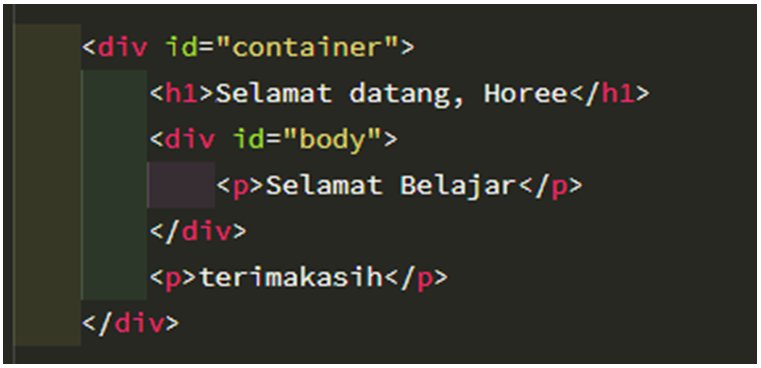
\includegraphics[width=0.80\textwidth]{figures/vs/15.png}}
	\caption{Contoh Penggunaan Indent-rainbow}
	\label{V15}
\end{figure}

pada gambar \ref{V15} tersebut merupakan source code CSS, dimana pada tag pembuka div pertama dapat di ketahui div penutupnya dengan tanda warna hujau transparan kemudian pada tag div ke dua juga dapat diketahui tag pembuka dan penutupnya melalui tanda warna ungu yang segaris dengan kedua tag tersebut.

\item Beautify\par
Digunakan untuk merapihkan code sehingga menjadi lebih teratur sebagai contoh seperti pada gambar \ref{V16} untuk source code yang tidak rapih sehingga menghasilkan source code yang rapih seperti pada gambar \ref{V17} 
 

\begin{figure}[!htbp]
	\centerline{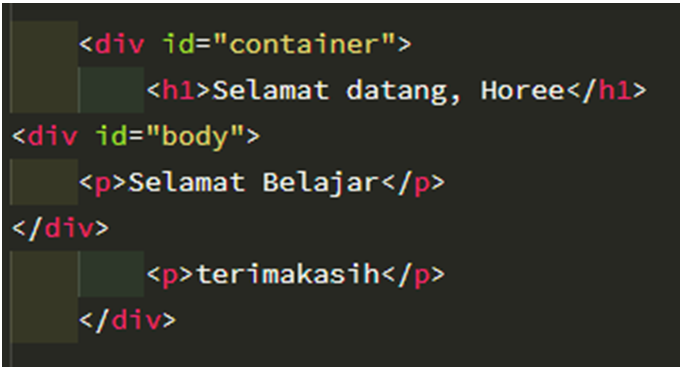
\includegraphics[width=0.90\textwidth]{figures/vs/16.png}}
	\caption{Souce code Acak}
	\label{V16}
\end{figure}

\begin{figure}[!htbp]
	\centerline{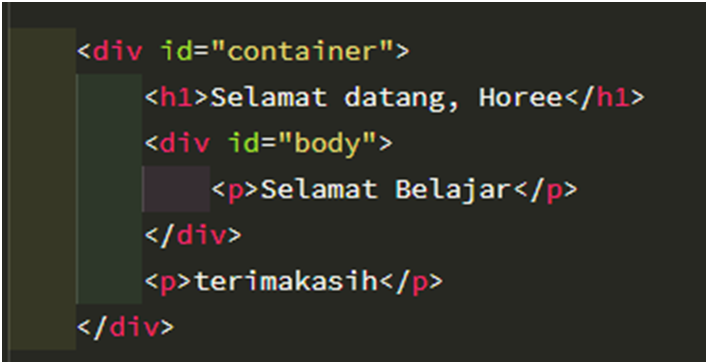
\includegraphics[width=0.90\textwidth]{figures/vs/17.png}}
	\caption{Source Code Rapih}
	\label{V17}
\end{figure}

berdasarkan pada gambar \ref{V16} dan gambar \ref{V17} untuk mengaktifkan ekstensi Beautify bisa di jalankan dengan cara menekan tombol ctrl dan S maka source code yang awalnya tidak beraturan akan menjadi rapih dan lebih tertata.


\item IntelliSense for CSS class names HTML\par
digunakan untuk mengkoreksi tag-tag dari CSS dan HTML, selain untuk mengkoreksi juga di gunakan untuk merekomendasikan Source code yang akan digunakan atau tag yang akan di gunakan. Misalkan progrmer akan menuliskan tag html, dengan menggunakan ekstensi tersebut cukup menuliskan tiga hurup tag pertama seperti <ht maka akan muncul rekomendasi tag html, jika telah muncul kemudian tekan enter maka secara otomatis tag pembuka dan penutup html jadi.
\item Material Icon Theme\par
Digunakan untuk memberikan icon pada folder atau file sesuai dengan fungsinya masing-masing misalkan seperti file php maka akan ada icon php begitupula file html maka akan memiliki icon html, agar lebih jelas maka hasilnya seperti pada gambar \ref{V18} berikut:
\begin{figure}[!htbp]
	\centerline{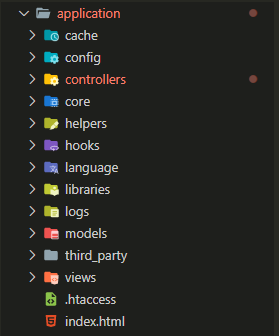
\includegraphics[width=0.45\textwidth]{figures/vs/18.png}}
	\caption{Menu Ekstensi Visual Studio}
	\label{V18}
\end{figure}
\item Monokai Theme\par
Merupakan ekstensi yang digunakan untuk merubah tema atau tampilan dari visual studio code, tampilan visual studio code jika menggunakan ekstensi ini akan seperti sublime text 3 dari tulisan hingga pewarnaan setiap tag source code,Bagi yang biasa menggunakan teks editor sublime text 3 dianjurkan untuk menggunakan ekstensi ini agar tampilan code menjadi seperti sublime text 3, sehingga menjadi pamiliar dan mempermudah dalam membuat sourcecode.

\pagebreak
\item PHP intellisense for codeigniter\par
Digunakan untuk mengkoreksi atau secara otomatis merekomendasikan code yang akan ditulis sesuai dengan librari codeigniter, misalkan menuliskan \$this-  maka akan ada rekomendasi tag penerusnya seperti input atau yang sejenisnya atau juga ketika memanggil sebuah model maka setelah menulis class model maka akan muncul rekomendasi fungsi-fungsi yang terdapat pada class pada model tersebut atau kasus lan seperti pada saat menuliskan ekstensi pada class maka akan muncul rekomendasi library yang akan di gunakan.\par


Sebagai alternatif untuk menerapkan ekstensi pada visual studio code bisa dengan cara memasukan source code tersebut pada settings.json yang terdapat  pada visual studio code, untuk lebih jelasnya berikut merupakan code yang harus di sesuaikan pada settings.json.

\end{enumerate}
\begin{lstlisting}[language=php]
{
    "workbench.colorTheme": "Monokai",
    "workbench.iconTheme": "material-icon-theme",
    "explorer.openEditors.visible": 0,
    "editor.minimap.enabled": false,
    "editor.lineHeight": 23,
    "editor.fontFamily": "'Source Code Pro',Consolas, 'Courier New', monospace",
    "terminal.integrated.shell.windows": "C:\\WINDOWS\\System32\\WindowsPowerShell\\v1.0\\powershell.exe",
    "php.suggest.basic": false,
    "editor.formatOnSave": true,
    "liveServer.settings.donotShowInfoMsg": true,
    "files.autoSave": "afterDelay"
}
\end{lstlisting} 

\section{ Instalasi \textit{CodeIgniter}}

Framework code igniter dapat di unduh website resminya yaitu www.codeigniter.com untuk tampilannya seperti pada gambar \ref{C1} beriku:\par
\begin{figure}[!htbp]
	\centerline{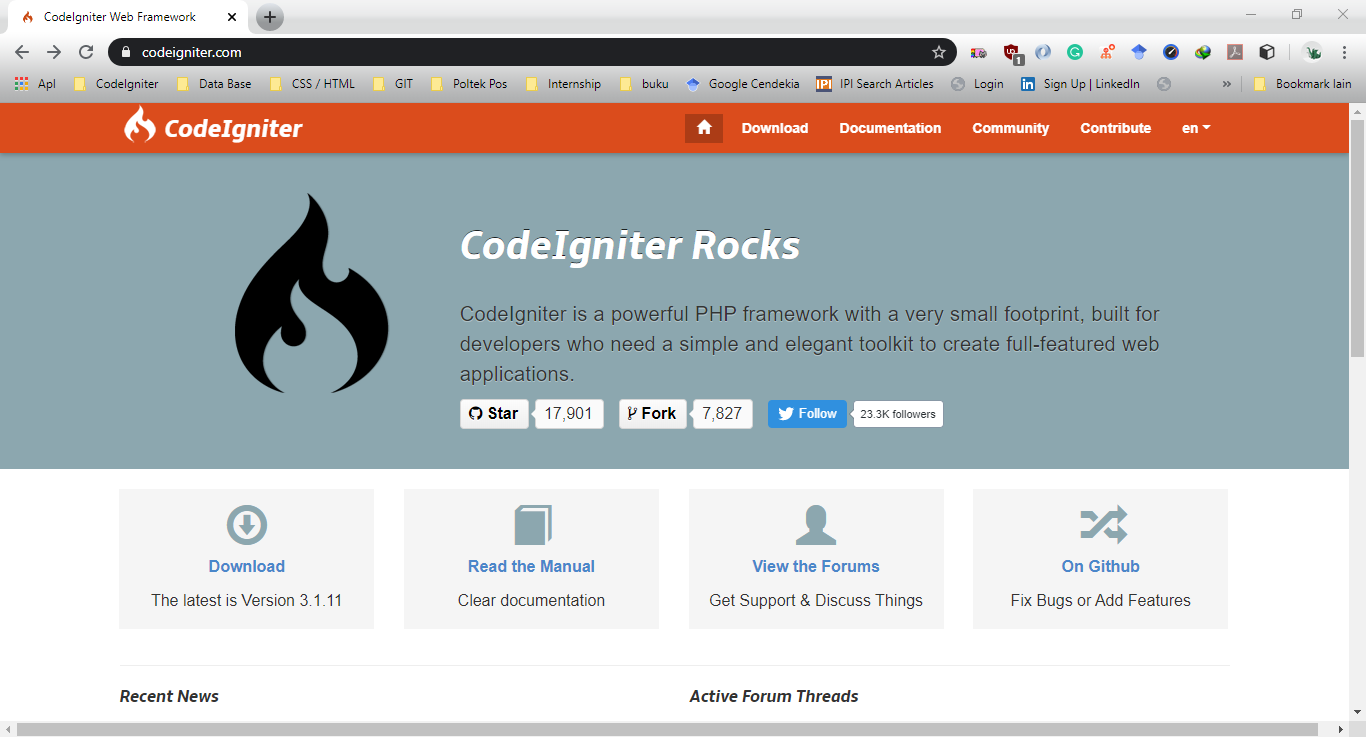
\includegraphics[width=1\textwidth]{figures/ci/1.png}}
	\caption{Tampilan Website CodeIgniter}
	\label{C1}
\end{figure}
Pada buku ini akan mengunakan codeigniter versi 3.1.11 yang terbaru pada saat buku ini di tulis. Untuk dapat mengunduhnya dapat menekean menu download yang terdapat pada halaman utama web resmi codeigniter atau dengan cara menekan menu download yang terdapat pada navigator bar maka akan pindah halaman ke halaman download pada halaman tersebut pilih menu codeigniter 3 dan download seperti pada gambar \ref{C2},
\begin{figure}[!htbp]
	\centerline{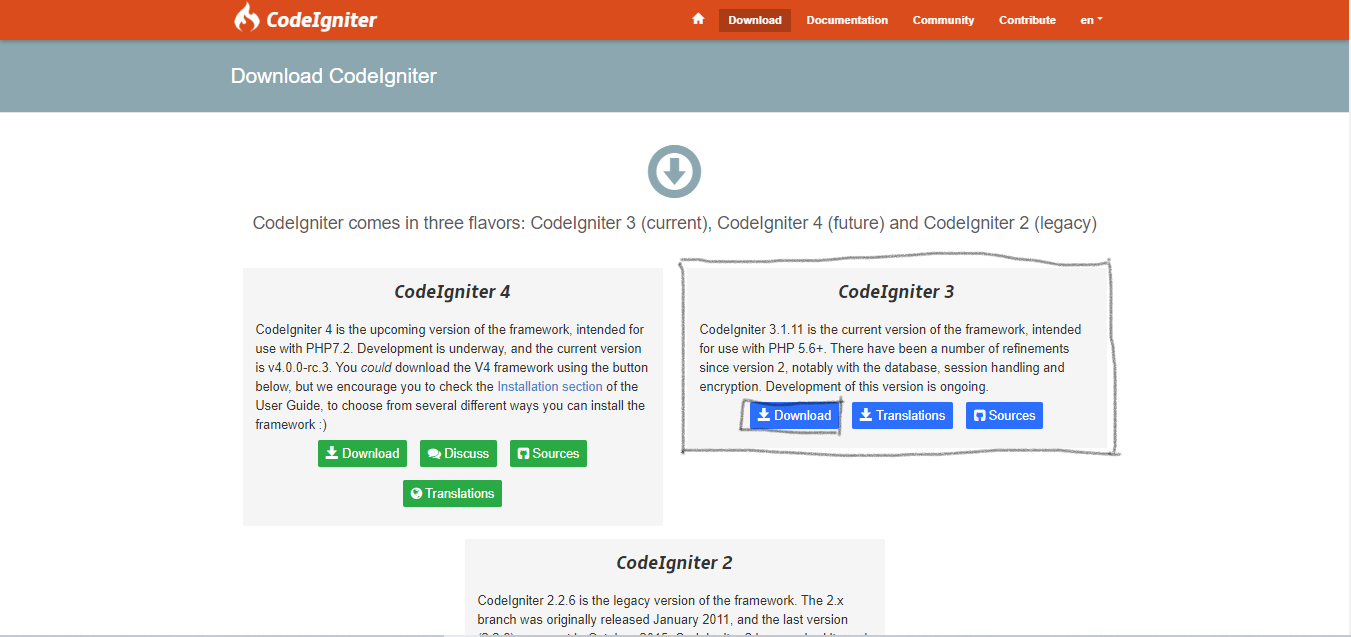
\includegraphics[width=1\textwidth]{figures/ci/2.png}}
	\caption{Halaman Download CodeIgniter}
	\label{C2}
\end{figure}
Setelah di unduh maka hasil file nya berupa zip dapat dilihat pada gambar \ref{C3}, setelah itu ekstrak file zip tersebut kemudian pindahkan ke direktori \begin{verbatim} C:\xampp\htdocs\end{verbatim} lalu agar mempermudah pemanggilan terhadap folder codeigniter bisa dilakukan dengancara mengganti nama folder codeigniter sebut misalkan menjadi CI sehingga hasilnya seperti pada gambar \ref{C4}.\par
\begin{figure}[!htbp]
	\centerline{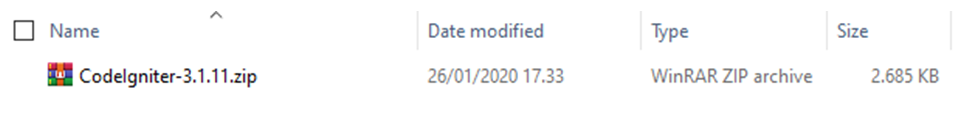
\includegraphics[width=1\textwidth]{figures/ci/3.png}}
	\caption{Hasil download file codeigniter}
	\label{C3}
\end{figure}
\begin{figure}[!htbp]
	\centerline{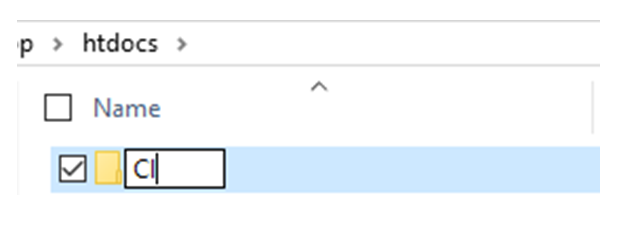
\includegraphics[width=0.85\textwidth]{figures/ci/4.png}}
	\caption{Folder CodeIgniter yang telah di rename}
	\label{C4}
\end{figure}
\pagebreak
Kemudian untuk memeriksa apakah codeigniter telah tepasang dengan benar atau belum dapat dilakukan dengan cara menuliskan alamat berikut :
 \begin{verbatim} http://localhost/CI \end{verbatim}

pada web browser yang di gunakan, jika codeignite rberjalan dengan baik maka hasilnya akan sepert pada gambar \ref{C5} berikut:
\begin{figure}[!htbp]
	\centerline{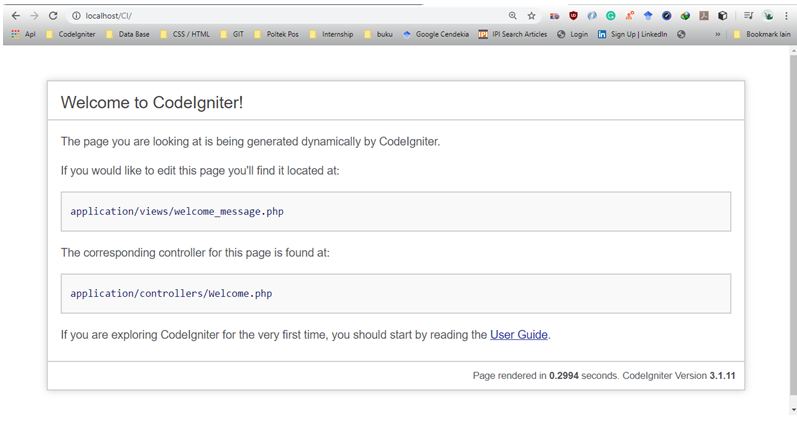
\includegraphics[width=1\textwidth]{figures/ci/5.png}}
	\caption{Hasil CodeIgniter}
	\label{C5}
\end{figure}
\subsection{Desain MVC}

Pada teknik pemerograman berorientasi objek, MVC atau model-view-controller merupakan sebuah metodelogi atau pola desain (desain pattern) yang digunakan untuk merelasikan data dan user interface dari suatu sistem agar menjadi efisien. Awalmulanya MVC digunakan untuk pemerograman berbasis dekstop khususnya untuk aplikasi-aplikasi yang di kembangkan menggunakan bahasa pemerograman C++, Java, dan Smalltalk, dengan semakin berkembangnya teknologi kini pengaplikasian model MVC tersebut diadopsi pada aplikasi yang berbasis web, sehingga hampir semua framework yang di gunakan untuk pengembangan web menggunakan konsep MVC \cite{raharjo2015belajar} .

Adapun komponen pada MVC dibagi menjadi tiga bagian yaitu:
\begin{enumerate}

\item Model yang berfungsi untuk mempresentasikan struktur data
\item View berfungsi untuk epresentasi keluaran atau output dari model yang berkaitan.
\item Controller  yang berpungsi untuk mengambil masukan dari user atau inputan dari user dan mengubahnya menjadi perintah untuk mengeksekusi model dan/atau view

\end{enumerate}

Umunya pola MVC dapat digambarkan seperti pada gambar \ref{C6} berikut :

\begin{figure}[!htbp]
	\centerline{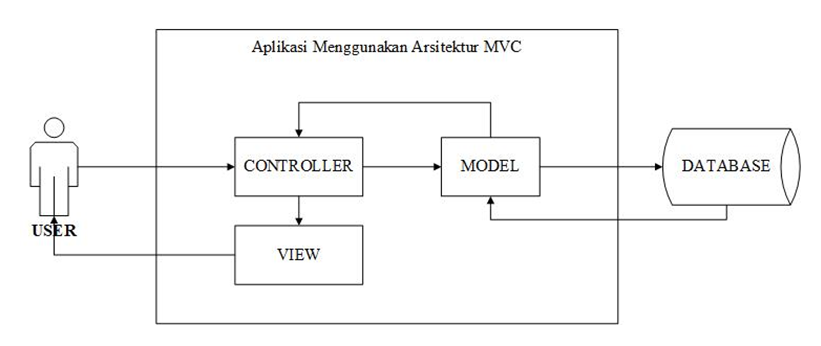
\includegraphics[width=1\textwidth]{figures/ci/6.png}}
	\caption{Alur Pola MVC Pada CodeIgniter}
	\label{C6}
\end{figure}

	pada gambar \ref{C6} tersebut dapat dijelaskan bahwa proses MVC dimulai dari aksi yang diberikan oleh user pengguna sistem kemudian aksi tersebut di terima oleh class dan method atau fungsi yang berangkutan pada controller  kemudian controller mengirim pesan ke model jika pada model tidak bersangkutan dengan basis data maka akan di kembalikan ke controller namun jika pada model bersangkutan dengan basis data maka fungsi pada model yang bersangkutan akan melakukan eksekusi pada data yang terdapat pada database tergantung pada fungsinya kemudian setelah itu data di kembalikan pada controller, kemudian controller menjalankan fungsi yang berkaitan dengan dta tersbut lalu mengirimkan data tersebut pada view yang menjadi user interface kepada user pengguna sistem.
\pagebreak

\subsection{Isi Folder CodeIgniter}

Isi folde atau susunan direktori pada codeigniter, pada satu paket codeigniter yang telah di download di dalammya terdapat tiga folder atau tiga direktori yaitu :
\begin{enumerate}
\item Apllication 
\item System 
\item User guide 
\end{enumerate}
Berikut merupakan penjelasan isi setiap folder yang terdapat pada satu paket codeigniter.


\subsection{Struktur Direktori Pada Folder Apllication}
Direktori application merupakan tempat file-file dari aplikasi yang akan dibuat. Berikut juga model MVC juga terdapat pada direktori ini. Kemudian jika ingin menambahkan fitur-fitur untuk aplikasi juga di simpan pada direktori ini, seperti template css javascrip, template HTML, dan file untuk eksport data, juga harus di simpan pada direktori ini. File-file tersebut di simpan pada folder atau subdirektori yang telah di sediakan oleh codeigniter itu sendiri.
Adapun daftar sub durektori yang terdapat pada direktori apllikasi seperti pada gambar \ref{C7} berikut:
\begin{figure}[!htbp]
	\centerline{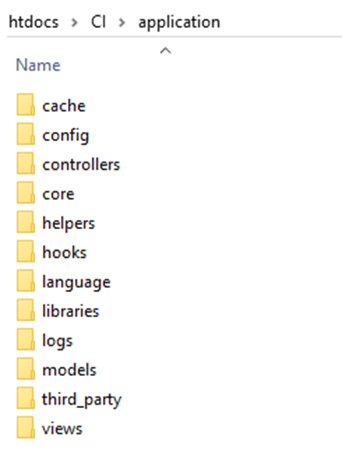
\includegraphics[width=0.40\textwidth]{figures/ci/7.png}}
	\caption{Isi Folder Apllication}
	\label{C7}
\end{figure}

Adapun penjelasan dari direktori pada gambar 16 tersebut sebagai berikut:
\begin{enumerate}
\item chace, digunakan untuk menyimpan halaman-halaman yang telah di buka sebelumnya kemudian di sembunyikan (chaced)
\item	config, berisikan file-file konfigurasi yang digunakan untuk aplikasi yang dibuat.
\item controller, berisi file-file controller dari aplikasi.
\item core, digunakan untuk menempatkan daftar file kelas dasar (base class) yang nantinya diturunkan pada class-class yang digunakan oleh aplikasi 
\item helpers, digunakan untuk menyimpan atau menempatkan file-file helper atau pustaka buatan sendiri yang di definisikan sendiri
\item hooks, berisi file pendukung aplikasi. Sebagai contoh, jika kita ingin memanggil suatu fungsi yang tersimpan di dalam file tertentu sebelum atau sesudah file controller dipanggil, maka dapat menempatkan file yang akan di eksekusi tersebut didalam sub direktori ini 
\item language, dalam direktori ini dapat mendefinisikan nilai konstanta-konstanta tertentu dalam bahasa yang diinginkan.
\item libraries, berisi daftar file library (pustaka dalam bentuk kelas yang di definisikan sendiri)
\item logs, digunakan oleh codeigniter untuk menyimpan logs (catatan) catatan yang secara otomatis ketika terjadi kesalahan.
\item models, berisi daftar file model yang di perlukan oleh aplikasi.
\item third party, digunakan untuk menyimpan plugin yang dikembangkan oleh pihak ketiga.
\item views, berisi file view yang digunakan oleh aplikasi.
\end{enumerate}

	
\subsection{Struktur Direktori Pada Folder System}
Pada direktori ini berisikan file-file yang telah di sediakan oleh codeigniter yang telah di kelasifikasikan berdasarkan fungsinya masing-masing, adapun sub kategori yang berada pada direktori system seperti pada gambar \ref{C8} berikut:

\begin{figure}[!htbp]
	\centerline{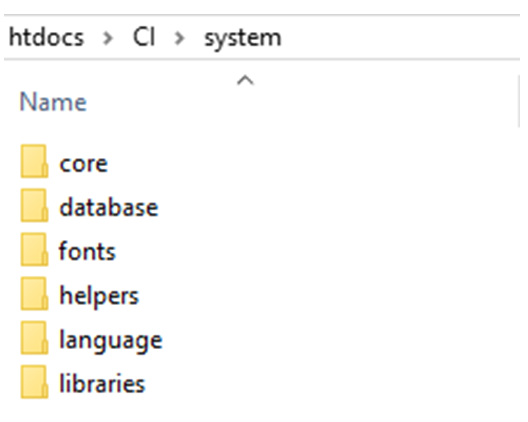
\includegraphics[width=0.40\textwidth]{figures/ci/8.png}}
	\caption{Isi Folder Apllication}
	\label{C8}
\end{figure}

\begin{enumerate}
\item core, berisikan file-file inti berupa class-class yang di gunakan oleh codeigniter, seperti CI\_Controller, CI\_Model dan lain-lain
\item database, berisikan file daftar file driver yang digunakan untuk mengakses database.
\item fonts, berisikan daftar file font 
\item helpers, berisi daftar file helper standar yang di sediakan oleh codeigniter.
\item language, berisi file-file bahasa (untuk keperluan translasi bahasa)
\item libraries, berisi daftar file daftar pustaka kelas standar yang di sediakan oleh codeigniter
\end{enumerate}

\subsection{Direktori user\_guide}
Direktori ini berisikan file-file dokumentasi penggunaan codeigniter dengan format file HTML direktori ini dapat tidakdi ikut sertakan dalam pembuatan aplikasi. Atau di cut keluar dari direktori temapt di codeugniter. Karena direktori ini tidak bepengaruh pada kedua direktori sebelumnya.

\section{Alur Aplikasi \textit{CodeIgniter}}

Adapun alur dari aplikasi yang ditulis menggunakan codeigniter digambarkan seperti pada gambar \ref{C9} berikut:\par
\begin{figure}[!htbp]
	\centerline{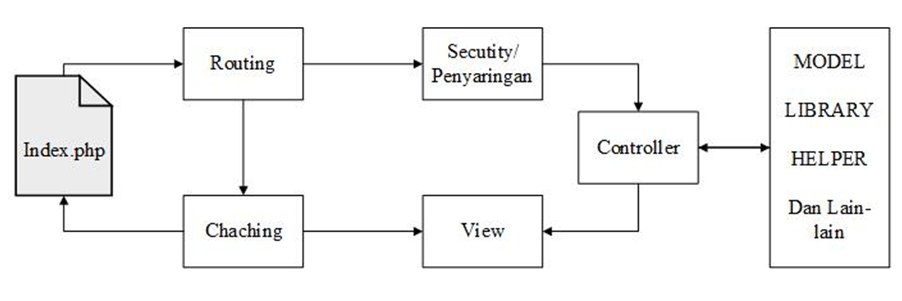
\includegraphics[width=1\textwidth]{figures/ci/9.png}}
	\caption{alur Aplikasi CodeIgniter}
	\label{C9}
\end{figure}

Alur pada gambar \ref{C9} tersebut dapat di jelaskan seperti berikut:
\begin{enumerate}
\item File index.php atau yang sering di sebut dengan entry script berperan sebagai controller depan, yang akan menginisialisasi daftar file yang dibutuhkan untuk menjalankan projek codeigniter. Dimana user melakukan perintah aplikasi ke server web melalui index.php, dengan format Unified Resource Identification (URI) seperti berikut :
\begin{verbatim}http://namahost/index.php/kelas-controller/fungsi  \end{verbatim} 
\item Permintaan yang dikirim oleh user berbentuk URI akan ditangkap oleh router, dan router akan menentukan controller dan metode mana yang harus di panggil
\item Jika ternyata halaman yang diminta oleh user telah di sembunyikan (chaced), halaman tersebut akan diambil dari chace dan langsung di sajikan kedalam web browser.
\item Sebelum controller yang diminta oleh user di eksekusi atau di muat, permintaan tersebut atau semua data yang dikirim oleh user akan di saring terlebih dahulu untuk keperluan pengamanan.
\item Controller akan memeuat model, library, herper, dan file-file yang diperlukan untuk memenuhi permintaaan user
\item Controller akan memuat view untuk di sajikan ke web browser jika mode chacing diaktifkan, maka view akan di caching terlebih dahulu sebelum ditampilkan, dengan demikian jika ada permintaan yang sama maka halaman tersebut tinggal di ambil melalui cache.
\end{enumerate}


\section{ Contoh MVC sederhana}

Aplikasi mengguanakan model MVC merupakan aplikasi yang lengkap, karena pada dasarnya jika menggunakan framework codeigniter maka harus menggunakan model MVC ini, untuk urutan contoh MVC adalah sebagai berikut:
\begin{enumerate}
\item Buat terlebih dahulu model untuk menyajikan data 
\item Buat controller untuk mengambil data dari model dan mengirimkan pada view 
\item Buat view untuk menampilkan data yang telah di kirim oleh controller.
\end{enumerate}
Untuk peroses dalam aplikasi tersebut adalah sebagai berikut:
\begin{enumerate}
\item Controller akan mengambil data yang terdapat pada model.
\item Model mengirimkan data sesuai dengan parameter yang diminta controller, parameter tersebut bisa berupa nama method dan atau variabel yang terdapat pada model
\item Kemudian pada controller ada perintah untuk menampilkan view dimana pada view tersebut akan mengambil data dari controller yang telah diambil dari model, dalam mengambil data biasanya dari controller di kirim menggunakan array assosiatif.
\item Maka view akan memperoses data yang di kirimkan oleh controller sehinga dapat di tampilkan hasil keluarannya sesuai dengan parameter yang digunakan pada controller.
\item Terakhir controller akan memperoses hasil yang ditampilkan oleh view ke layar web browser.
\end{enumerate}
Agar dapat memulai contoh MVC pada codeigniter buka folder codeigniter mengguanakan visual studio code seperti pada gambar \ref{mvc1} berikut:

\begin{figure}[!htbp]
	\centerline{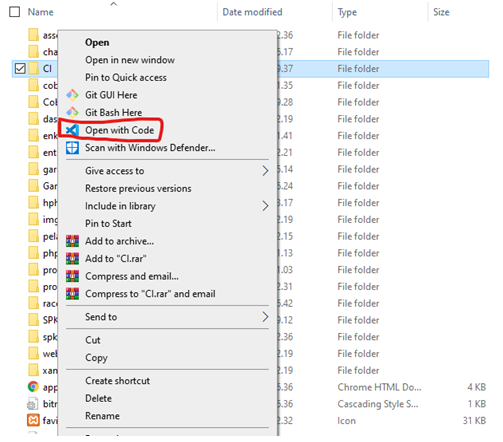
\includegraphics[width=0.80\textwidth]{figures/MVC/1.png}}
	\caption{Open With Visual Code}
	\label{mvc1}
\end{figure}
\pagebreak
%ada gambar

Pada gambar \ref{mvc1} merupakan cara untuk membuka folder codeigniter menggunakan visual studio code untuk hasilnya seperti pada gambar \ref{mvc2} berikut:

\begin{figure}[h]
	\centerline{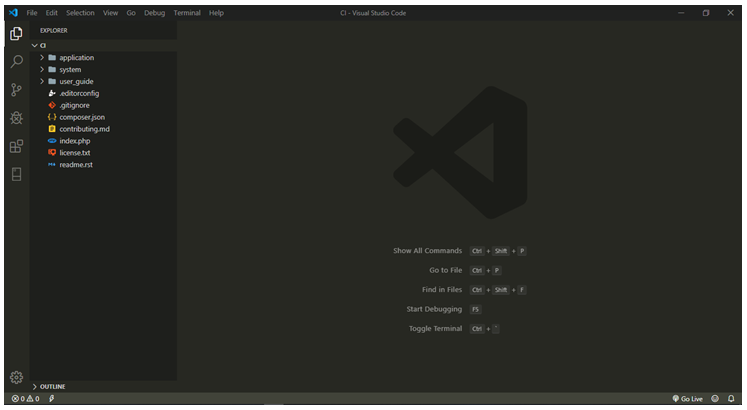
\includegraphics[width=0.95\textwidth]{figures/MVC/2.png}}
	\caption{Folder CodeIgniter Menggunakan}
	\label{mvc2}
\end{figure}
%ada gambar

Pada gambar \ref{mvc2} tampilan direktori code yang di buka menggunakan visual studio code. Setelah tampilannnya seperti pada gambar \ref{mvc2} klik direktori application kemudian pilih sub direktori model sehingga tampilannya seperti pada gambar \ref{mvc3}

\begin{figure}[h]
	\centerline{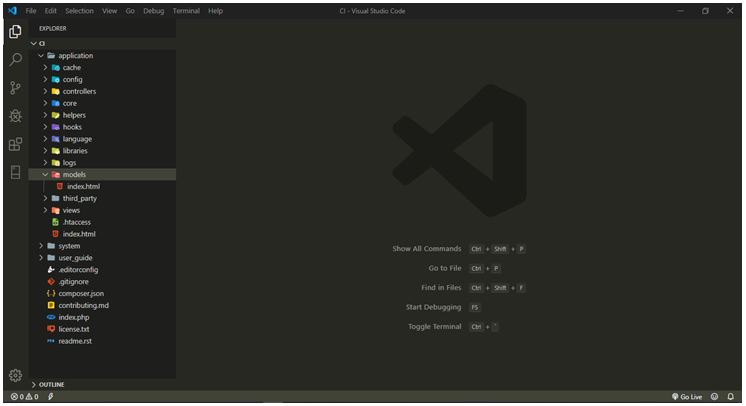
\includegraphics[width=0.95\textwidth]{figures/MVC/3.png}}
	\caption{Direktori Applications}
	\label{mvc3}
\end{figure}
\pagebreak
%ada gambar

Setelah muncul seperti pada gambar \ref{mvc3} kemudian  klik kanan pada sub direktori models kemudian pilih new file dan beri nama model\_mvc.php sehingga hasilnya seperti pada gambar \ref{mvc4} berikut.
\begin{figure}[h]
	\centerline{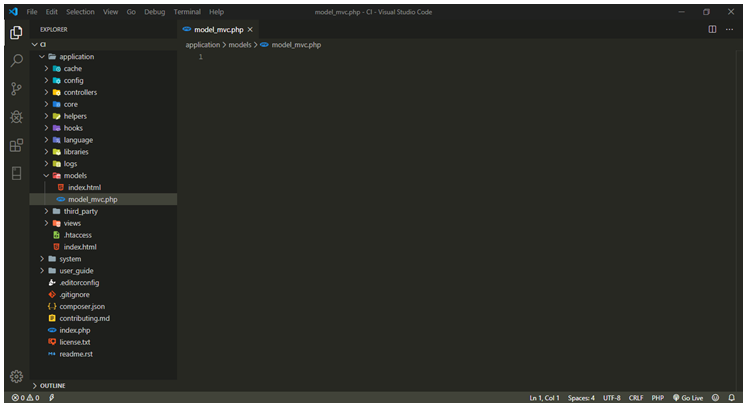
\includegraphics[width=0.95\textwidth]{figures/MVC/4.png}}
	\caption{Membuat File Mode\_mvc}
	\label{mvc4}
\end{figure}
%ada gambar

Jika telah muncul tampilan seperti pada gambar 39 maka masukan codingan berikut pada file model\_mvc.php

\begin{lstlisting}[language=PHP]
<?php
class Model_mvc extends CI_Model
{
    // membuat variabel atau properti dengan nama $str dengan tipe data string
    public $str = 'Mencoba CodeIgniter';
}

\end{lstlisting} 
\textbf{Penjelasan \textit{Source Code}}.\par
	Untuk membuat model hal seperti kode diatas yaitu:
\begin{enumerate}
\item buat tag php pada baris pertama, hal ini dilakukan karena base dari Codeigniter sendiri merupakan PHP
\item pada baris ke dua buat class dengan nama class yang harus sama dengan nama file model hanya hanyasaja pada hurup pertama harus kapital, jika nama filenya \textbf{model\_mvc.php} berarti nama kelasnnya harus \textbf{Model\_mvc}, kemudian harus eksten ke class CI\_Model dikarenakan source code tersebut merupakn model.
\item untuk isi source code pada class tersebut harus di tempatkan di dalam kurung kurawal yang terdapat pada baris ke tiga dan enam pada source code tersebut.
\item pada baris ke empat merupakan comment pada source code tanda coment itu sendiri yaitu garis miring duakali sebelum source code, lalu comment ini tidak akan di tampilkan atau di eksekusi oleh sistem.
\item pada baris ke 5 merupakan variabel atau properti yang berisikan data string kemudian berstatus public yang berarti variabel tersebut bisa di akses oleh class lain.
\end{enumerate}

Setelah memasukan codingan tersebut buat Controller dengan nama Controller\_mvc.php dengan cara klik kanan sub direktori controllers kemudian buat file baru dengan memilih new file kemudian berinama Controller\_mvc.php. maka hasilnya seperti pada gambar \ref{mvc5} berikut

\begin{figure}[h]
	\centerline{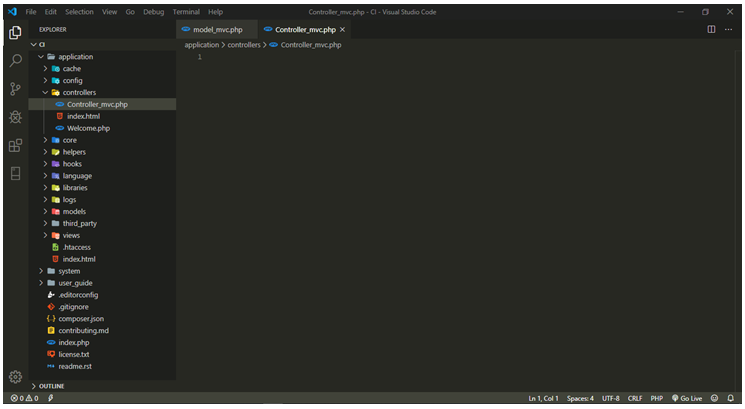
\includegraphics[width=0.95\textwidth]{figures/MVC/5.png}}
	\caption{Membuat File Controller\_mvc}
	\label{mvc5}
\end{figure}

%ada gambar

Jika telah muncul tampilan seperti pada gambar \ref{mvc5} maka masukan codingan berikut pada file Controller\_mvc.php
\begin{lstlisting}[language=PHP]
<?php
class Controller_mvc extends CI_Controller
{
    public function index()
    {
        // memanggil atau memuat 'model_mvc'
        $this->load->model('model_mvc');
        // mengambil objek dari krlas model_mvc'
        // yang dimasukan ke variabel $data_model
        $data_model = $this->model_mvc;
        // mengambil data yang terdapat pada model
        $string = $data_model->str;
        // membuat inisial data yang di kirim ke view
        $data['data'] = $string;
        // menampilakan dan mengirimkan data ke view
        $this->load->view('view_mvc', $data);
    }
}

\end{lstlisting} 
\pagebreak
\textbf{Penjelasan \textit{Source Code}}.\par
	pada dasarnya pembuatan file dan source code pada controller hampir mirip dangan model, untuk penjelasan source code tersebut sebagai berikut:
\begin{enumerate}
\item pada baris pertama ada tag PHP karena basenya sama menggunakan PHP.
\item kemudian pada baris ke dua buat class Controller\_mvc, sama seperti model nama class harus sama dengan nama file hanyasaja pada controller nama file harus di dahului dengan huruf kapital dan nama class harus didahului dengan huruf kapital, kemudian ekstensinya ke class CI\_Controller dikarenakan file controller dan terdapat pada folder controller.
\item pada baris ke tiga dan 18 merupakan kurung kurawal pembuka dan penutup dari class, yang merupakan tanda bahwa source code yang di buat pada class tersebut harus berada di dalam kurung kurawal tersebut.
\item pada baris ke empat merupakan fungsi index yang merupakan fungsi yang harus ada pada controller karena fungsi yang pertama di jalankan ketika memanggil controller tersebut merupakan fungsi index 
\item pada baris ke lima dan ke 17 merupakan kurung kurawal pembuka dan penutup pada fungsi tersebut yang berarti fungsi tersebut akan menjalankan program yang terdapat pada kurung kurawal tersebut 
\item kemudian untuk source code yang berwarna hijau atau ada sesuadah garismiring duakali // merupakan comment dari source code.
\item pada baris ke tujuh merupakaan source code untuk memuat model pada fungsi tersebut, adapun pada source code tersebut model yang di muat yaitu (model\_mvc) yang telah di buat pada folder model tadi.
\item pada baris ke 10 membuat variabel baru dengan nama data\_model yang di gunakan untuk menampung model\_mvc dan objeknya. 
\item pada baris ke 12 merupakan source code untuk mengambil data dari model dengan cara memasukan pada variabel baru bernama string, setelah itu di isi dengan variabel yang di dalamnya tardapat model\_mvc setelah itu dilanjutkan dengan memanggil objek atau pungsi yangterdapat pada model, pada contoh tersebut yang di panggil merupakan objek bernama (str).
\item membuat array assosiatif yang dibuat dengan variabel data kemudian di isi dengan variabel string.
\item pada baris ke 16 merupakan kode untuk menampilkan view kemudian di iringi dengan variabel data yang di gunakan untuk mengirim data ke view tersebut.
\end{enumerate}
\pagebreak

Setelah file controller di buat dan di isikan codingan tersebut maka selanjutnya buat tampilan atau view yang bertujuan untuk di tampilkan pada web browser dengan nama view\_mvc.php, untuk caranya yaitu pilih sub direktori views kemudian klik kanan pilih new file kemudian berinama view\_mvc yang hasilnya seperti pada gambar \ref{mvc6} berikut

\begin{figure}[h]
	\centerline{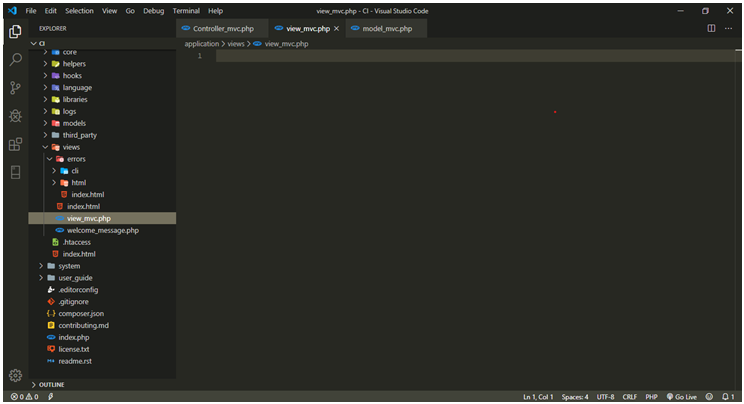
\includegraphics[width=0.95\textwidth]{figures/MVC/6.png}}
	\caption{Membuat File view\_mvc}
	\label{mvc6}
\end{figure}
%ada gambar

Jika tempilannya telah sama atau mirip seperti pada gambar \ref{mvc6} maka masukan code berikut pada file view\_mvc.php. walaupun ekstensi pada file tesebut merupakan php tapi isi code didalammnya merupakan tag HTML dikarenakan di gunakan untuk tampilan sehingga bisa lebih menarik.
\begin{lstlisting}[language=HTML]
<html>
<head>
    <title>
        contoh pemerograman mvc
    </title>
</head>
<body>
    <h3>
        <?php echo $data; ?>
    </h3>
</body>

</html>
\end{lstlisting}
\pagebreak
\textbf{Penjelasan \textit{Source Code}}.\par

Pada source code tersebut menggunakan tag html diakarenakan digunakan untuk menampilkan data yang telah di tampilkan controller. adapun penejelasan file view tersebut sebagai berikut:
\begin{enumerate}
\item file view dibuat dengan ekstensi php bukan html, dikarenakan codeigniter menggunakan base Php sehingga untuk view menggunakan ekstensi php hal ini bertujuan agar file view tersebut dapat dieksekusi atau di jalankan oleh controller.
\item pada baris ke satu dan 13 merupakan tag html
\item pada baris ke dua dan ke 6 merupakan tag head.
\item pada baris ke tiga dan lima merupakan tag title.
\item pada baris ke tujuh dan ke 11 merupakan tag body html 
\item kemudian pada body terdapat tag header tiga dan pada baris ke 4 merupakan variabel data yang merupakan parameter dari controller yang di kirim menggunakan array assosiatif. 
\end{enumerate}

Kemudian untuk menjalankan hasil dari codingan controller model dan view tersebut nyalakan terlebih dahulu xampp yaitu dengan menyalakan xampp control panel dan memilih start pada apache dan mysql, setelah itu buka web browser kemudian isikan alamat tersebut http://localhost/CI/index.php/Controller\_mvc maka hasilnya seperti pada gambar \ref{mvc7} berikut.

\begin{figure}[h]
	\centerline{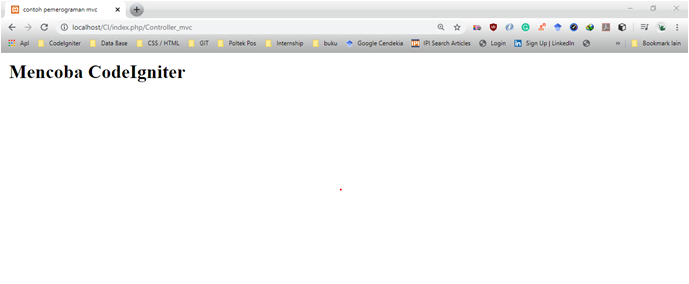
\includegraphics[width=0.95\textwidth]{figures/MVC/7.png}}
	\caption{view contoh mvc sederhana}
	\label{mvc7}
\end{figure}
%ada gambar

\pagebreak
	pada file view tersebut di dapat dikombinasikan  dengan bahasa pemrograman lain seperti css dan javascript,hal ini bisa dilakukan dengan cara menuliskan langsung source code css atau java script tersebut pada file tersebut atau bisa di lakukan dengan cara menimpan file css dan java script pada folder lain kemudian nanti pada tag html di panggil pada bagian header atau footer.
berikut ini merupakan source code untuk view yang di padukan dengan css, pada source code tersebut source code css di tuliskan pada file pada view.
\begin{lstlisting}[language=PHP]
<?php
defined('BASEPATH') or exit('No direct script access allowed');
?>
<!DOCTYPE html>
<html lang="en">

<head>
    <meta charset="utf-8">
    <title> contoh pemerograman mvc </title>

    <style type="text/css">
        ::selection {
            background-color: #E13300;
            color: white;
        }

        ::-moz-selection {
            background-color: #E13300;
            color: white;
        }

        body {
            background-color: #fff;
            margin: 40px;
            font: 13px/20px normal Helvetica, Arial, sans-serif;
            color: #4F5155;
        }

        a {
            color: #003399;
            background-color: transparent;
            font-weight: normal;
        }

        h1 {
            color: #444;
            background-color: transparent;
            border-bottom: 1px solid #D0D0D0;
            font-size: 19px;
            font-weight: normal;
            margin: 0 0 14px 0;
            padding: 14px 15px 10px 15px;
        }

        code {
            font-family: Consolas, Monaco, Courier New, Courier, monospace;
            font-size: 12px;
            background-color: #f9f9f9;
            border: 1px solid #D0D0D0;
            color: #002166;
            display: block;
            margin: 14px 0 14px 0;
            padding: 12px 10px 12px 10px;
        }

        #body {
            margin: 0 15px 0 15px;
        }

        p.footer {
            text-align: right;
            font-size: 11px;
            border-top: 1px solid #D0D0D0;
            line-height: 32px;
            padding: 0 10px 0 10px;
            margin: 20px 0 0 0;
        }

        #container {
            margin: 10px;
            border: 1px solid #D0D0D0;
            box-shadow: 0 0 8px #D0D0D0;
        }
    </style>
</head>

<body>

    <div id="container">
        <h1>Belajar Codeigniter MVC</h1>
        <div id="body">
            <p><?php echo $data ?></p>
        </div>
    </div>

</body>

</html>

\end{lstlisting} 
\pagebreak
\textbf{Penjelasan \textit{Source Code}}.\par
pada source code tersebut di gunakan untuk view pada dasarnya seperti php view seperti biasa, kemudian untuk menyisipkan source code atau link untuk memanggil css di tuliskan pada bagian header, atau pada source code tersebut pada baris ke tujuh samapai baris ke 76, lalu untuk source code tersebut merupakan css bawaan dari codeigniter.

Untuk hasinya seperti pada gambar \ref{mvc7} seperti berikut:

\begin{figure}[h]
	\centerline{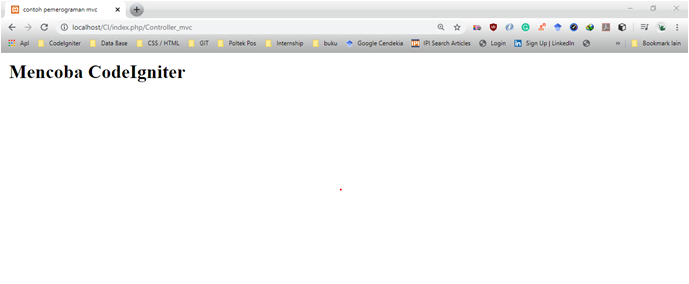
\includegraphics[width=0.95\textwidth]{figures/MVC/7.png}}
	\caption{view contoh mvc sederhana}
	\label{mvc7}
\end{figure}
 
%ada gambar


\section{ Penjelasan Mengirim data MVC}

Pada konsep mvc dikarenakan menggunakan class sehingga konsep turunan dari kelas pasti digunakan atau secara intinya konsep OOP sengat digunakan. Untuk itu berikut penjelasan cara mengirimkan data menggunakan konsep MVC pada codeigniter 
	Pada code model di contoh implementasi MVC terdapat code berikut:\par

\begin{lstlisting}[language=PHP]
public $str = ‘Mencoba CodeIgniter’ 
\end{lstlisting}
Source code tersebut merupakan objek sebagai variabel str dengan isi data string (Mencoba CodeIgniter) yang mana objek tersebut berstatus public yang berarti dapat di gunakan oleh class lain, sehingga jika data tersebut akan di ambil atau di gunakan pada controller harus mendekralasikan terlebih dahulu class dari model tersebut, contohnya yaitu seperti pada file Controller\_mvc terdapat source code seperti berikut.
\begin{lstlisting}[language=PHP]
$this->load->model(‘model_mvc’);
\end{lstlisting} 
Code tersebut berarti memanggil atau memuat model dari folder model dengan nama class dan file ‘model\_mvc’ code tersebut dapat di sisipkan pada setiap fungsi pada class yang berada pada controller, atau jika model tersebut di gunakan oleh banyak fungsi atau dominasi fungsi dapat menuliskannya pada pungsi konstruktor, kemudian untuk contoh menyisipkan code untuk memuat model seperti code tersebut:
\begin{lstlisting}[language=PHP]
    public function get_data()
    {
        $this->load->model('model_mvc');
        // code yang berkaitan dengan model
    }

\end{lstlisting} 
Yang di maksud contruktor yaitu fungsi yang di gunakan untuk meload atau memuat model, library dari codeigniter kemudian model atau library tersebut dapat di gunakan pada fungsi-fungsi yang terdapat pada class tersebut untuk contoh penulisan construktor, yaitu seperti pada source code berikut:
\begin{lstlisting}[language=PHP]
function __construct()
	{
		parent::__construct();
		$this->load->model('model_mvc');
	}

\end{lstlisting}  
Setelah meload atau memanggil model maka setiap fungsi dan objek yang berstatus public dapat di gunakan pada controller, pada contoh implementasi MVC tersebut yaitu menggunakan objek str untuk menggunakan data di dalammnya. Untuk dapat menggunakan atau memanggil data pada objek dapat dilakukan dengan cara seperti pada code berikut:
\begin{lstlisting}[language=PHP]
$data_model = $this->model_mvc;
$string = $data_model->str;

\end{lstlisting}

Pada variabel \$data\_model yang memuat model\_mvc kemudian untuk mengambil fungsi yang berada pada model dapat menggunakan vfariabel baru pada contoh terbut yaitu \$string dengan isi variabel \$data\_model kemudian merujuk pada str yang merupakan objek yang terdapat pada model. Selain menggunakan code tersebut dapat dilakukan seperti code tersebut sehingga menjadi lebih sederhana.

\begin{lstlisting}[language=PHP]
$string = $this->model_mvc->str
\end{lstlisting}
source code tersebut intinya sama yaitu mengambil data pada objek str yang terdapat pada file model\_mvc. Kemudian untuk mengirimkan data tersebut pada view harus menggunakan array asosiatif atau data harus berupa objek pada code implementasi MVC menggunakan code berikut 

\begin{lstlisting}[language=PHP]
$data['data'] = $string;
\end{lstlisting}

Variabel \$string merupakan data yang di kirim ke view yang berisikan data objek str dari model, code untuk mengirim data juga dapat di tuliskan seperti berikut: 

\begin{lstlisting}[language=PHP]
$data = array('data' => $string);
\end{lstlisting}

Atau bisa juga sebagai berikut

\begin{lstlisting}[language=PHP]
$data = ['data' => $string]
\end{lstlisting}

Code tersebut dapat diimplementasikan pada php 5.4 atau versi di atasnya.
Untuk mengirimkan data tersebut pada view dilakukan pada saat memuat view yaitu dengan menjadikan variabel \$data menjadi parameter seperti pada code berikut

\begin{lstlisting}[language=PHP]
$this->load->view('view_mvc', $data);
\end{lstlisting}

Berdasarkan code tersebut maka code tersebut juga dapat di ruliskan seperti berikut:

\begin{lstlisting}[language=PHP]
$this->load->view(‘view_mvc’, array('data' => $string));
\end{lstlisting}
atau
\begin{lstlisting}[language=PHP]
$this->load->view(‘view_mvc’, ['data' => $string]);
\end{lstlisting}

data merupakan kunci dari array asosiatif yang digunakan untuk memanggil data pada view yaitu dengan cara merubanya menjadi variabel yaitu dengan menambahkan tanda seperti berikut(\$) sebagai contoh pada view dapat di panggil seperti berikut  

\begin{lstlisting}[language=PHP]
<?php echo $data ?>
\end{lstlisting}
Atau 
\begin{lstlisting}[language=PHP]
<?= $data ?>
\end{lstlisting}
\begin{lstlisting}[language=PHP]

\end{lstlisting}
%\ref{lst:flcs}:
%\lstinputlisting[caption=File flasklivechart.py,label={lst:flcs}]{src/mia.py}









